\documentclass{article}
\usepackage{graphicx} % Required for inserting images

\title{CTA200 - Final Project - MW Analogues in cosmological simulations}
\author{Anagha Samaga}
\date{May 2026}

\begin{document}

\maketitle
\newpage

\section{ Introduction}

To understand how galaxies form and evolve,  complex physical processes like gas accretion, star formation, and feedback from supernovae and active galactic nuclei (AGN) are studied. Since, these mechanisms happen across massive timescales, cosmological  simulations are used to track how matter distributes itself and to test our theoretical models against real observations. A key relation  used to study this is the "galaxy star formation main sequence" , which plots a galaxy's total stellar mass $M_*$ against its current star formation rate $M_*$. This  relation demonstrates  how different "sub-grid" physical prescriptions alter how galaxies shut down their star formation and become quiescent, "red and dead" systems. This project compares these behaviors across two major simulation frameworks: the EAGLE simulation suite and the IllustrisTNG project.

To carry out this comparison, Python pipelines were created to interface directly with both simulation databases. For the EAGLE data, the script connects to the VirgoDB database using \verb|eagleSqlTools| to run a structured SQL query, pulling the stellar masses and star formation rates for all resolved subhalos in the largest 100 Mpc volume at the final snapshot ($SnapNum = 28$, which corresponds to redshift $z=0$). For IllustrisTNG, the data is pulled from the TNG100-1 web API using HTTP GET requests ($Snapshot = 99$, $z=0$). Since requesting millions of records at once causes the server to time out, a previous datafile containing the data was used. Finally, the data was processed with \verb|numpy| and plotted using \verb|matplotlib| to produce log-log scatter plots exported in PDF format, allowing for a direct comparison of the physical behaviors modeled by each simulation 

\newpage
\section{Project Sections}

1. Retrieving EAGLE Galaxy properties: your first SQL query in python

2. Going Deeper into the Simulations: more properties and more snapshots

3. Another Simulation: Querying data from IllustrisTNG

\newpage
\subsubsection{Retrieving EAGLE Galaxy properties: your first SQL query in python}


To analyze the galaxy star formation main sequence, automated data retrieval pipelines were developed in Python to interface with the simulation databases. For the EAGLE simulation data, a secure connection was established to the remote VirgoDB server using the eagleSqlTools library. A structured SQL query was executed to filter and download properties from the flagship 100 Mpc box ($RefL0100N1504_SubHalo$), extracting the stellar mass and star formation rate  for all resolved subhalos at the present-day universe snapshot ($SnapNum = 28$, corresponding to redshift $z=0$). 

\begin{figure}
    \centering
    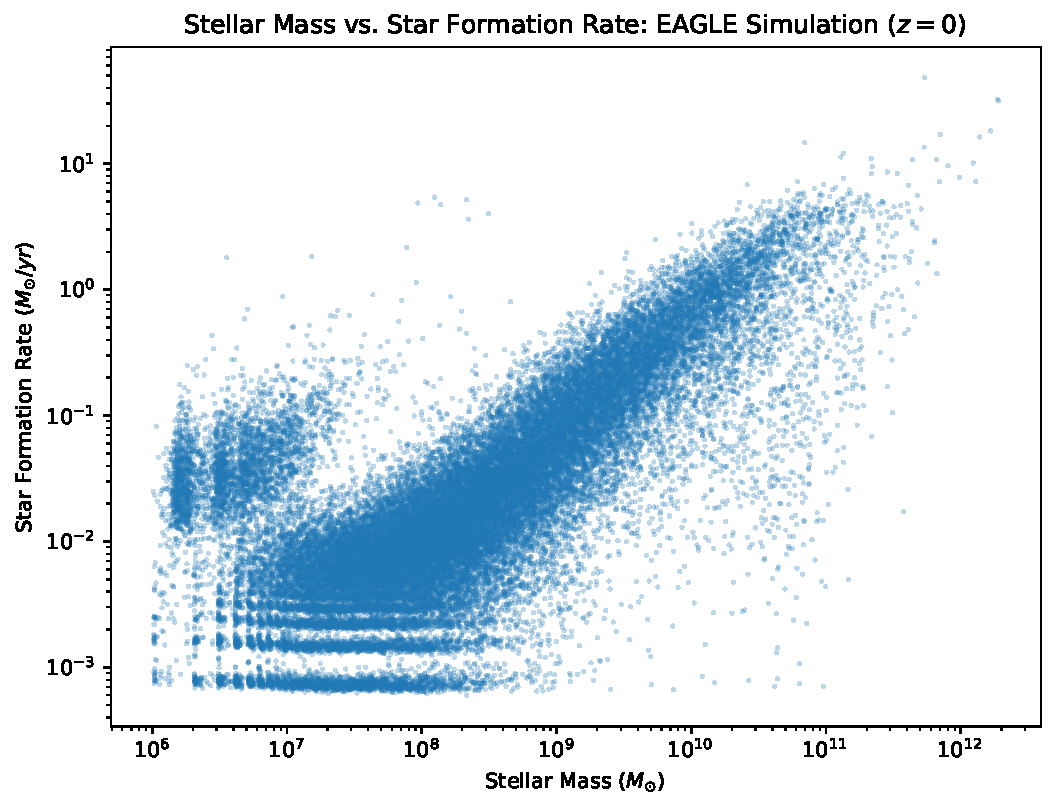
\includegraphics[width=0.5\linewidth]{eagle_sfr_vs_mass.pdf}
    \caption{EAGLE Simulation Data Plot}
    \label{fig:placeholder}
\end{figure}

The query retrieves the total mass of all stars within the galaxy and their star formation rate for each of the galaxies from the 28th "Snapshot" which represents a redshift of 0. The condition placed on the query is too only pull the data from the 28th snapshot, which means that the data from the simulation represents data from a redshift of 0. This means that the results will be from the simulations from the "present day". The same constraint can be made using the column "Redshift" and requesting only data where Redshift = 0.0.


The data was then plotted using Matplotlib, resulting in Figure 1. In Figure 1, we can see that there is a clear correlation between Stellar Mass and the SFR, where more massive galaxies have higher SFR. 

SFR  $\propto \ $ Stellar  Mass

There is a "floor" at lower Stellar Masses and SFRs, with small gaps in the data, creating lines. For masses less than $10^{10.5}$ but more than $10^{9.5}$ solar masses, AGN feedback might exhibit lower SFRs due to quenching. For galaxies with larger masses than $10^{10.5}$ solar masses, most galaxies are most likely already quenched, causing a lack of trends. Key differences from observations of nature include over-quenching at low masses where the simulation has a lack of data but where dwarf galaxies should still be star-forming and the "lines" rather than gradual transitions. These may arise as simulations use discrete large timesteps that skip stages lasting only a few Myrs. This computational 'shortcut' is how large cosmological volumes are simulated on practical timescales instead of tracking every stage.
\newpage
\subsubsection{Going Deeper into the Simulations: more properties and more snapshots}

In order to view a wider range of outputs, a second sequel query was made in order to get galaxies with redshifts ranging from 0.0 (present day) to 0.5.  Matplotlib was used again to create a plot of the Stellar Mass versus the Star Formation Rate. We can clearly see that  there is a significantly larger amount of galaxies in this output compared to the first section (10x) and the Main Sequence is denser (Figure 2). Two changes in distributions include the Main Sequence being denser and broader, with more scattering vertically on the edges of the sequence compared to the first sequence, and the Main Sequence being shifted upwards, with more galaxies with high SFRs and Stellar Masses compared to the first section. 

\begin{figure}
    \centering
    \includegraphics[width=0.5\linewidth]{EAGLESIM2.png}
    \caption{EAGLE Simulation Stellar Mass SFR Main Sequence}
    \label{Figure 2. EAGLE Simulation Stellar Mass SFR Main Sequence}
\end{figure}

When we observe the universe using telescopic data, we see galaxies across a range of redshifts as light from distant galaxies takes large amounts of time to reach us, and hence we see the galaxies as they were when the light left the galaxy. As a result, this is more representative of what we would see in an observational galaxy survey as it collects data from varying time periods, which represents the real variation on redshifts we observe. The maximum redshift a survey can observe is determined by how faint galaxies become with distance, as since as galaxies get farther away, they become dimmer due to light spreading out and the loss of redshift, so surveys are limited by their instrument sensitivity until galaxies become too faint to detect.


\newpage
\subsubsection{
Another Simulation: Querying data from IllustrisTNG}

For the IllustrisTNG simulation data, an API-driven retrieval pipeline was initially created to interface with the TNG100-1 web database at present-day redshift $z=0$. A custom helper function was structured to handle secure header authentication using an API key and to automatically parse incoming JSON payloads. Initial  queries to retrieve the subhalo data returned metadata with a total population of 4,371,211  subhalos. However, trying to query and download this entire dataset by setting the API payload length to the total galaxy count (\verb|limit=n_gal|)  resulted in a network timeout error due to the computational limits of delivering millions of records at once. To avoid this  limitation, the API pipeline was not used in favor of direct local file. A pre-compiled data file (\verb|data_all.npy|) containing the complete  dictionary array of IllustrisTNG subhalo properties was sourced locally from the CITA cluster storage network (\verb|/mnt/raid-cita/savelli/|). This file was linked directly into the notebook, with instant data extraction of the star formation rates and stellar masses required.  Matplotlib was used again to create a plot of the Stellar Mass versus the Star Formation Rate.
\begin{figure}
    \centering
    \includegraphics[width=0.5\linewidth]{The ILLU.png}
    \caption{IllustrisTNG Simulation Stellar Mass SFR Main Sequence}
    \label{fig:3}
\end{figure}

There are major differences between this plot and the ones made using the EAGLE data as the Main Sequence is more dense in the middle of the sequence with high scattering compared to the EAGLE plot (Figure 3). This may be attributed to the lower stellar masses, as the stellar masses range mostly from 10\^-2 to 10\^2 whereas the EAGLE stellar masses range from 10\^6 to 10\^12. Beyond the units, the physical behavior of the "red and dead" galaxies look different. In EAGLE, there is a distinct empty gap right below the main sequence, showing that the galaxies quench and stop forming stars very rapidly. In TNG, that space has a dense, continuous cloud of transitioning galaxies, implying quenching is a much more gradual process in this simulation. Finally, at the high-mass end, TNG’s main sequence bends downward and scatters much more aggressively than EAGLE's. This might be due to how it models the Active Galactic Nuclei (AGN) feedback (as mentioned in previous sections).

\newpage

\section{References}

Dylan Nelson for the TNG Collaboration. (n.d.). \textit{TNG}. IllustrisTNG - Project Description. https://www.tng-project.org/about/ 

Matthee, J., \& Schaye, J. (2019). The origin of scatter in the star formation rate–Stellar Mass relation. \textit{Monthly Notices of the Royal Astronomical Society}, \textit{484}(1), 915–932. https://doi.org/10.1093/mnras/stz030 

McAlpine, S., Helly, J. C., Schaller, M., Trayford, J. W., Qu, Y., Furlong, M., Bower, R. G., Crain, R. A., Schaye, J., Theuns, T., Dalla Vecchia, C., Frenk, C. S., McCarthy, I. G., Jenkins, A., Rosas-Guevara, Y., White, S. D. M., Baes, M., Camps, P., \& Lemson, G. (2016). The Eagle Simulations of Galaxy Formation: Public release of Halo and Galaxy Catalogues. \textit{Astronomy and Computing}, \textit{15}, 72–89. https://doi.org/10.1016/j.ascom.2016.02.004 

Proctor, K. (n.d.). \textit{The galaxy main sequence: What’s in the scatter? | Astrobites}. Astrobites. https://astrobites.org/2021/01/30/galaxy-ms-scatter/ 

Whitaker, K. E., van Dokkum, P. G., Brammer, G., \& Franx, M. (2012). The star formation mass sequence out to                    \textit{z}                    = 2.5. \textit{The Astrophysical Journal}, \textit{754}(2). https://doi.org/10.1088/2041-8205/754/2/l29 


\end{document}

